\vspace{1em}

\usetikzlibrary{graphs, positioning, quotes, shapes.geometric}

\begin{document}
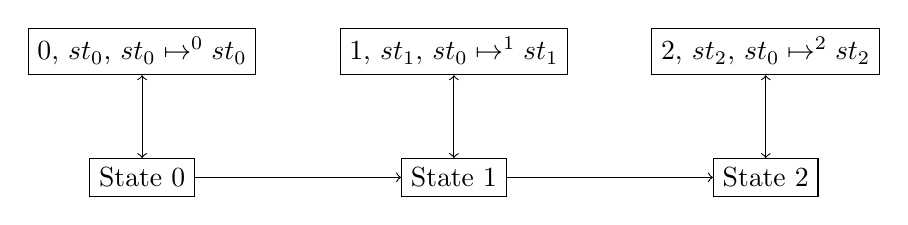
\begin{tikzpicture}[node distance=10pt]
    \node[draw] (Description 0)  {0, $st_{0}$, $st_{0}\mapsto^{0}st_{0}$};
    \node[draw, right=30pt of Description 0] (Description 1)  {1, $st_{1}$, $st_{0}\mapsto^{1}st_{1}$};
    \node[draw, right=30pt of Description 1] (Description 2)  {2, $st_{2}$, $st_{0}\mapsto^{2}st_{2}$};
    
    \node[draw, below=30pt of Description 0]    (State 0)  {State 0};
    \node[draw, below=30pt of Description 1]    (State 1)  {State 1};
    \node[draw, below=30pt of Description 2]    (State 2)  {State 2};
    

    \graph{
        (State 0) -> (State 1) -> (State 2);
        (State 0) <-> (Description 0);
        (State 1) <-> (Description 1);
        (State 2) <-> (Description 2);
    };
\end{tikzpicture}